\documentclass{article}
\usepackage{graphicx, amssymb}
\usepackage{amsmath}
\usepackage{amsfonts}
\usepackage{amsthm}
\usepackage{kotex}
\usepackage{bm}
\usepackage{hyperref}
\usepackage{xcolor}
\usepackage{mathrsfs}
\usepackage{tikz-cd}
\usepackage{mathtools}
\usepackage{physics}

\textwidth 6.5 truein 
\oddsidemargin 0 truein 
\evensidemargin -0.50 truein 
\topmargin -.5 truein 
\textheight 8.5in

\DeclareMathOperator{\cc}{\mathbb{C}}
\DeclareMathOperator{\rr}{\mathbb{R}}
\DeclareMathOperator{\bA}{\mathbb{A}}
\DeclareMathOperator{\fra}{\mathfrak{a}}
\DeclareMathOperator{\frb}{\mathfrak{b}}
\DeclareMathOperator{\frm}{\mathfrak{m}}
\DeclareMathOperator{\frp}{\mathfrak{p}}
\DeclareMathOperator{\slin}{\mathfrak{sl}}
\DeclareMathOperator{\Lie}{\mathsf{Lie}}
\DeclareMathOperator{\Alg}{\mathsf{Alg}}
\DeclareMathOperator{\Spec}{\mathrm{Spec}}
\DeclareMathOperator{\End}{\mathrm{End}}
\DeclareMathOperator{\rad}{\mathrm{rad}}
\newcommand*\Laplace{\mathop{}\!\mathbin\bigtriangleup}
\newcommand{\id}{\mathrm{id}}
\newcommand{\Hom}{\mathrm{Hom}}
\newcommand{\Sch}{\mathbf{Sch}}
\newcommand{\Ring}{\mathbf{Ring}}
\newcommand{\T}{\mathcal{T}}
\newcommand{\B}{\mathcal{B}}
\newcommand{\Mod}[1]{\ (\mathrm{mod}\ #1)}
\newtheorem{lemma}{Lemma}
\newtheorem{theorem}{Theorem}
\newtheorem{proposition}{Proposition}
\def\Xint#1{\mathchoice
{\XXint\displaystyle\textstyle{#1}}%
{\XXint\textstyle\scriptstyle{#1}}%
{\XXint\scriptstyle\scriptscriptstyle{#1}}%
{\XXint\scriptscriptstyle\scriptscriptstyle{#1}}%
\!\int}
\def\XXint#1#2#3{{\setbox0=\hbox{$#1{#2#3}{\int}$ }
\vcenter{\hbox{$#2#3$ }}\kern-.6\wd0}}
\def\ddashint{\Xint=}
\def\dashint{\Xint-}

\tikzset{
    rotate around with nodes/.style args={#1:#2}{
        rotate around={#1:#2},
        set node rotation={#1},
    },
    rotate with/.style={rotate=\qrrNodeRotation},
    set node rotation/.store in=\qrrNodeRotation,
}

\usetikzlibrary{calc,angles,quotes,positioning,datavisualization, patterns}

\def\tickheight{2pt}
\def\tickamount{4}

\begin{document}


\title{Partial Differential Equation - HW 1}
\author{SungBin Park, 20150462} 

 \maketitle

\section*{Problem 1}
\begin{enumerate}
\item[(a)] \begin{equation*}
\begin{split}
&\int_{\partial B_r(x)}\nabla \Phi_y (y-x)\cdot \bm{\nu}_{out}dS_y\\
&=-\int_{\partial B_r(x)}\frac{1}{2\pi}\left(\frac{y_1-x_1}{(y_1-x_1)^2+(y_2-x_2)^2}, \frac{y_2-x_2}{(y_1-x_1)^2+(y_2-x_2)^2}\right)\cdot\\
&~~~~~~~~~~~~~~~~~~~~~\left(\frac{y_1-x_1}{\sqrt{(y_1-x_1)^2+(y_2-x_2)^2}}, \frac{y_2-x_2}{\sqrt{(y_1-x_1)^2+(y_2-x_2)^2}}\right)dS_y\\
&=-\frac{1}{2\pi}\int_0^{2\pi}d\theta=-1.
\end{split}
\end{equation*}
\item[(b)]
\begin{equation*}
\begin{split}
-\Laplace(\Phi*f)&=-\Laplace\left(\int_{\rr^2}\Phi(x-y)f(y)dy\right)=-\Laplace\left(\int_{\rr^2}\Phi(y)f(x-y)dy\right) \text{ (By change of variable)}\\
&=-\int_{\rr^2}\Phi(y)\Laplace_x f(x-y)dy=-\int_{\rr^2}\Phi(y)\Laplace_y f(x-y)dy\\
&=-\left(\int_{\rr^2 \setminus B_\epsilon(0)}\Phi(y)\Laplace_y f(x-y)dy+\int_{B_\epsilon(0)}\Phi(y)\Laplace_y f(x-y)dy\right)=J_\epsilon+I_\epsilon.
\end{split}
\end{equation*}
But,
\begin{equation*}
\abs{I_\epsilon}\leq \norm{D^2 f}_{L^\infty(\rr^2)}\int_{B_\epsilon(0)}\Phi(y)dy\leq\norm{D^2 f}_{L^\infty(\rr^2)}\frac{1}{2}\epsilon^2\log{\epsilon}.
\end{equation*}
Therefore, $I_\epsilon\rightarrow 0$ as $\epsilon\rightarrow 0$.

In $\rr^n\setminus B_\epsilon(0)$, $\Phi(y)$ is smooth, so we can use integration by part and green's formula
\begin{equation*}
\begin{split}
J_\epsilon &=-\int_{\rr^n\setminus B_\epsilon(0)}\nabla\cdot(\Phi(y)\nabla f)-\nabla\Phi(y)\cdot\nabla f(x-y)dy \\
&=-\int_{\rr^n\setminus B_\epsilon(0)}\nabla\cdot(\Phi(y)\nabla f)-\nabla\Phi(y)\cdot\nabla f(x-y)dy \text{ (integration by part)}\\
&=-\int_{\partial B_\epsilon(0)}\Phi(y)\frac{\partial f}{\partial\bm{\nu}}(x-y) dS_y+\int_{\rr^n\setminus B_\epsilon(0)}\nabla\Phi(y)\cdot\nabla f(x-y)dy \text{ (Using green's formula)}\\
&=K_\epsilon+L_\epsilon.
\end{split}
\end{equation*}
The $\bm{\nu}$ represents the outward normal vector of $\partial \rr^n\setminus B_\epsilon(0)$, which is inner normal vector of $\partial B_\epsilon(0)$. But,
\begin{equation*}
\abs{K_\epsilon}\leq \norm{Df}_{L^\infty(\rr^n)}\int_{\partial B_\epsilon(0)}\abs{\Phi(y)}dS_y\leq\norm{Df}_{L^\infty(\rr^n)}\epsilon\abs{\log\epsilon}.
\end{equation*}
Therefore, $K_\epsilon\rightarrow0$ as $\epsilon\rightarrow0$.
Finally, using integration by part,
\begin{equation*}
\begin{split}
L_\epsilon &=\int_{\rr^n\setminus B_\epsilon(0)}\nabla\cdot(\nabla\Phi(y) f)-f(x-y)\Laplace\Phi(y)dy \\
&=\int_{\partial B_\epsilon(0)} f(x-y)\pdv{\Phi(y)}{\bm{\nu}}dS_y \text{ (since }\Phi(y) \text{ is harmonic away from 0)} \\
&=\int_{\partial B_\epsilon(x)} f(x)\pdv{\Phi(y-x)}{\bm{\nu}}dS_y
\end{split}
\end{equation*}
Since $f$ is continuous and $\int_{\partial B_\epsilon(0)} \pdv{\Phi(y)}{\bm{\nu}}dS_y=1$ for all $\epsilon>0$,(note that $\bm{\nu}$ is inward normal vector, contributing $-$ sign.) $\int_{\partial B_\epsilon(x)} f(y)\pdv{\Phi(y-x)}{\bm{\nu}}dS_y\rightarrow f(x)$ as $\epsilon\rightarrow 0$.
\end{enumerate}
\section*{Problem 2}
\begin{enumerate}
\item[(i)$\Rightarrow$(ii)]
Let's use change of variable that $y=x+rz$, then
\begin{equation}\label{Eq:2-1}
\dashint_{\partial B_r(x)}u(y)dS_y=\dashint_{\partial B_1(0)}u(x+rz)dS_z.
\end{equation}
Let $\phi(r)$ be \eqref{Eq:2-1}, then
\begin{equation*}
\phi'(r)=\dashint_{\partial B_1(0)}\nabla u(x+rz)\cdot z dS_z.
\end{equation*}
Restoring the variable $y$,
\begin{equation}\label{Eq:2-2}
\begin{split}
\phi'(r)=\dashint_{\partial B_r(x)}u(y)\cdot \frac{y-x}{r}dS_y&=\dashint_{\partial B_r(x)}\pdv{u}{\bm{\nu}}dS_y\\
&=\frac{r}{n}\dashint_{\partial B_r(x)}\Laplace u(y)dy=0.
\end{split}
\end{equation}
Therefore, $\phi(r)$ is constant function, and so
\begin{equation*}
\phi(r)=\lim\limits_{r\rightarrow0}\dashint_{\partial B_r(x)}u(y)dS_y=u(x)~\forall r>0
\end{equation*}
since $u$ is continuous on $\overline{B_r(x)}\subset \Omega$.
\item[(ii)$\Rightarrow$(iii)] Using polar coordinate,
\begin{equation*}
\int_{B_r(x)}u(y)dy=\int_0^r \left(\int_{\partial B_t(x)}u dS\right) dt=\int_0^r nt^{n-1}w_n u(x) dt=r^n w_n u(x)
\end{equation*}
where $w_n$ is the volume of unit ball in $\rr^n$. Hence, $\dashint_{B_r(x)}u(y)dy=u(x)$.
\item[(iii)$\Rightarrow$(ii)] Using polar coordinate,
\begin{equation*}
\dv{r}\int_0^r \left(\int_{\partial B_t(x)}u dS\right)dt=\int_{\partial B_r(x)}u dS=nr^{n-1}w_nu(x)
\end{equation*}
Therefore, $\dashint_{\partial B_r(x)}u(y) dS_y=u(x)$.
\item[(ii)$\Rightarrow$(i)] Let $\Laplace u\neq 0$. Since $u\in C^2(\Omega)$, there exists an $B_r(x)$ such that $\Laplace u(y)>0$ in the ball.(If $\Laplace u\leq 0$, then change $u$ to $-u$)

Then, by \eqref{Eq:2-2}
\begin{equation*}
\phi'(r)=\frac{r}{n}\dashint_{\partial B_r(x)}\Laplace u(y)dy>0
\end{equation*}
and it is impossible to satisfy (ii).
\end{enumerate}
\section*{Problem 3}
Since $A$ is symmetric, positive definite matrix, there exists eigendecomposition $U\Lambda U^T$, where all the eigenvalue of $\Lambda$ is positive and $U$ is orthogonal real matrix. Let the diagonal value of $\Lambda$ $\lambda_i$, and $\bm{\xi}_i$ be the corresponding eigenvector. If we construct $v=\sum_{i=1}^n \sqrt{\lambda_i^{-1}}\bm{\xi}_i$, then $vv^T=A^{-1}$.

Let 
\begin{equation*}
t_i=\sqrt{\lambda_i}^{-1} \bm{\xi}_i^T \bm{x}=\sqrt{\lambda_i}^{-1}\begin{bmatrix}
\xi_{i1} & \xi_{i2} & \cdots &\xi_{in}
\end{bmatrix}
\begin{bmatrix}
x_{1} \\ x_{2} \\ \vdots \\ x_{n}
\end{bmatrix}=\sqrt{\lambda_i}^{-1}\sum\limits_{j=1}^n \xi_{ij}x_j.
\end{equation*}
Then,
\begin{equation}\label{Eq:3-1}
x_i=\sum\limits_{j=1}^n \sqrt{\lambda_j}\xi_{ji}t_j.
\end{equation}
Using \eqref{Eq:3-1}, 
\begin{equation*}
\pdv{u}{t_i}=\sum_{j=1}^n \pdv{u}{x_j}\pdv{x_j}{t_i}=\sum_{j=1}^n \sqrt{\lambda_i}\xi_{ij}\pdv{u}{x_j}
\end{equation*}
and
\begin{equation*}
\frac{\partial^2 u}{\partial t_i \partial t_i}=\sum_{k=1}^n \sum_{j=1}^n \sqrt{\lambda_i}\xi_{ij}\frac{\partial^2 u}{\partial x_k \partial x_j}\pdv{x_k}{t_i}=\sum_{k=1}^n \sum_{j=1}^n \sqrt{\lambda_i\lambda_i}\xi_{ij}\xi_{ik}\frac{\partial^2 u}{\partial x_k \partial x_j}.
\end{equation*}
Summing up by $i$,
\begin{equation*}
\sum\limits_{i=1}^n\frac{\partial^2 u}{\partial t_i^2}=\sum_{k=1}^n \sum_{j=1}^n a_{jk}\frac{\partial^2 u}{\partial x_k \partial x_j}.
\end{equation*}
Since $U$ is orthogonal matrix, it spans $\rr^n$, and we can get $\Laplace_t u=0$.
\begin{enumerate}
\item[(a)] Let $\Omega'=A\Omega=\{Ax|x\in \Omega\}$ and $u(t(x))=u(Ax)$. Since $A$ is a bicontinuous linear function sending $x$ to $t$, it preserves open, bounded, and connected property. Also, it preserves derivative property, so $u(t)\in C^2(\Omega')\cap C(\overline{\Omega'})$.

Let there exists a maximum point $x_0\in \Omega$ such that $u(x_0)=M=\max\limits_{\overline{\Omega}}u$. If $x_0\in \Omega$, $t_0 \in \Omega'$, and it means $u(t)$ is constant in $\Omega'$ by the proof of strong maximum principle, implying $u(x)$ is constant in $\Omega$. Hence,
\begin{equation*}
\max_{\overline{\Omega}}u=\max_{\partial \Omega}u.
\end{equation*}
\item[(b)] Let $\Omega'_*=A\Omega_*$. As I stated above, $\Omega'_*$ is open, bounded, and connected. Also, $\overline{\Omega'_*}$ is compact since it is a image of continuous function, satisfying $\Omega'_*\subset\overline{\Omega'_*}\subset \Omega'$.

By Harnack's ineuqality, 
\begin{equation*}
\sup_{\Omega'_*}u(t)\leq C\inf_{\Omega'_*}u(t)
\end{equation*}
for some constant $C$ only depends on $n$, $\Omega'$ and $\Omega'_*$.

Since $\sup_{\Omega'_*}u(Ax)=\sup_{A^{-1}\Omega'_*}u(x)=\sup_{\Omega_*}u(x)$, and $\inf_{\Omega'_*}u(Ax)=\inf_{\Omega_*}u(x)$. Let $\lambda=\min\{\lambda_i\}$, where $\lambda_i$ are the eigenvalues of $A$. Then, the number of balls in $\overline{\Omega'_*}$ is at most number of balls in $\overline{\Omega_*}$ times $\lceil\lambda\rceil^{-n}$. Therefore, $C$ depends on $n$, $\Omega$ and $\Omega_*$.
\end{enumerate}

\section*{Problem 4}
\begin{enumerate}
\item[(a)] Let $\phi(r)=\dashint_{\partial B_r(x)}v(y)dS_y=\dashint_{\partial B_1(0)}v(x+rz)dS_z$. Then
\begin{equation*}
\begin{split}
\phi'(r)&=\dashint_{\partial B_1(0)}\nabla v(x+rz)\cdot\bm{z}dS_z=\dashint_{\partial B_1(0)}\nabla v(x+rz)\cdot\bm{z}dS_z\\
&=\dashint_{\partial B_r(x)}\nabla v(y)\cdot\frac{y-x}{r} dS_y=\dashint_{\partial B_r(x)}\pdv{v}{\bm{\nu}}dS_y=\frac{r}{n}\dashint_{\partial B_r(x)} \Laplace v dS_y\geq 0~\text{ (By Green's theorme)}
\end{split}
\end{equation*}
So, $\phi(r)$ is a decreasing function. Letting $r\rightarrow 0$, $\dashint_{\partial B_r(x)}v(y)dS_y\rightarrow v(x)$ since $v\in C^2(\overline{\Omega})$. Therefore, for all $r$ and $x\in \Omega$, $\dashint_{\partial B_r(x)}v(y)dS_y\geq v(x)$. Also, using polar coordinate
\begin{equation*}
\dashint_{B_r(x)} v(y)dy=\frac{1}{w_n}\int_0^r\int_{\partial B_t(x)} v(y)dS_y dt\geq v(x)\frac{1}{w_n}\int_0^r \sigma(S^{n-1}(t))dt=v(x)
\end{equation*}
where $\sigma(S^{n-1}(t))$ is the area of a sphere of dimension $n-1$ with radius $t$. Hence, 
\begin{equation*}
v(x)\geq\dashint_{B_r(x)}v(y)dy
\end{equation*}
\item[(b)] Let $x_0$ be a maximum point in $\Omega$ and $M=v(x_0)$. Then, there exists $r>0$ such that $B_r(x_0)\in \Omega$. Then, $M=v(x_0)\leq\dashint_{B_r(x_0)}v(y)dy\leq M$ since $v(y)\leq M$. Since $v(y)$ is continuous and $v(y)=M$ almost everywhere in $B_r(x_0)$, $v(y)=M$ in  $B_r(x_0)$. $v^{-1}(M)$ is closed since $v$ is continuous, and $v^{-1}(M)$ is open since it have neighborhood for each point. Hence, $v^{-1}(M)$ is whole set if $U$ is connected, and it means $v$ is constant function, implying $\max\limits_{\overline{\Omega}}v=\max\limits_{\partial \Omega} v$.

If $v$ is not a constant function, then $v$ should not have maximum on $\Omega$. Hence, $v$ should have maximum on $\partial \Omega$, and $\max\limits_{\overline{\Omega}} v=\max\limits_{\partial \Omega}v$.
\item[(c)] 
\begin{equation*}
\begin{split}
\Laplace \abs{Du}^2&=\sum\limits_{j=1}^n \partial^2_{x_j}\left(\sum\limits_{i=1}^n (\partial_{x_i} u)^2\right)\\
&=\sum\limits_{j=1}^n\left(\sum\limits_{i=1}^n 2(\partial_{x_i} u)(\partial_{x_j x_j x_i} u)+2(\partial_{x_j x_i})^2\right)\\
&=\sum\limits_{j=1}^n 2(\partial_{x_j x_i}u)^2 \text{ (Since } \sum\limits_{i=1}^n\partial_{x_j x_j}u=\Laplace u=0\text{ in } \Omega \text{)}\\
&\geq 0.
\end{split}
\end{equation*}
Therefore, $\abs{Du}^2$ is subharmonic, and by (b),
\begin{equation*}
\max_{\overline{\Omega}}\abs{Du}^2=\max_{\partial \Omega}\abs{Du}^2.
\end{equation*}

\section*{Problem 5}
Let $u'=\pm u+\frac{|x|^2}{2n}\max\limits_{\overline{\Omega}}\abs{f}$, then
\begin{equation*}
-\Laplace u'=-\Laplace (\pm u)-\max\limits_{\overline{\Omega}}\abs{f}=\pm f-\max\limits_{\overline{\Omega}}\abs{f}\leq 0.
\end{equation*}
Therefore, we can use subharmonic property of $u'$. Using strong maximum principle for subharmonic fun function,(with $u'\in C^2(\Omega)\cap C^0(\overline{\Omega})$)
\begin{equation*}
\max\limits_{\overline{\Omega}}u'=\max{\pm u}+\max\limits_{\overline{\Omega}} \left(\frac{|x|^2}{2n}\max\limits_{\overline{\Omega}}\abs{f}\right)=\max\limits_{\partial \Omega} \left(\pm u+\frac{|x|^2}{2n}\max\limits_{\overline{\Omega}}\abs{f}\right)\leq\max\limits_{\partial \Omega} (\pm g)+\frac{R^2}{2n}\max\limits_{\overline{\Omega}}\abs{f}
\end{equation*}
where $R>0$ is a constant satisfying $\Omega\subset B_R(0)$ sincfe $\Omega$ is bounded. Summarising above equation,
\begin{equation*}
\max\abs{u}\leq \max\limits_{\partial \Omega} \abs{g}+\frac{R^2}{2n}\max\limits_{\overline{\Omega}}\abs{f}\leq C\left(\max_{\partial\Omega}\abs{g}+\max_{\overline{\Omega}}\abs{f}\right)
\end{equation*}
for some constant only depends on $\Omega$ and dimension $n$.

\section*{Problem 6}
I'll first show that $u\in C^\infty(\Omega)$ if $u$ satisfies mean-value property and boundedness of derivative of $u$, and then I'll show $u$ is analytic.
\begin{lemma}
If $u\in C(\Omega)$ satisfies mean-value property for each ball $B_r(x)$ for all $x\in \Omega$, then $u$ is smooth in $\Omega$.
\end{lemma}
\begin{proof}
Let $\eta$ be a standard modifier. For example, we can set $\eta$ by
\begin{equation*}
\eta(x)\coloneqq
\begin{cases}
C\exp\left(\frac{1}{\abs{x}^2-1}\right) & \text{if }\abs{x}<1 \\
0 & \text{if } \abs{x}\geq 1
\end{cases}
\end{equation*}
the constant $C>0$ is taken to be $\int_{\rr^n} \eta dx=1$. For $\epsilon>0$, we can define
\begin{equation*}
\eta_\epsilon(x)\coloneqq \frac{1}{\epsilon^n}\eta\left(\frac{x}{\epsilon}\right)
\end{equation*}
Then, $\eta_\epsilon\in C^\infty$ and
\begin{equation*}
\int_{\rr^n} \eta_\epsilon dx=1,~\text{spt}(\eta_\epsilon)\subset B_\epsilon(0)
\end{equation*}
Let $\Omega_\epsilon=\{x\in \Omega | \text{dist}(x,\partial \Omega)>\epsilon\}$ and set $u_\epsilon(x)\coloneqq \eta_\epsilon*u=\int_{\Omega}\eta_\epsilon(x-y)u(y)dy$ in $\Omega_\epsilon$. Since $u$ is continuous function, it is known that $u_\epsilon(x)\in C^\infty(\Omega_\epsilon)$.(The differentiation about $x$ affect only on $\eta_\epsilon(x-y)$, and because $\eta_\epsilon(x-y)$ have good property, $\pdv{u_{\epsilon}}{x_i}=\int_{\Omega}\frac{\partial \eta_{\epsilon}}{\partial x_i}(x-y)u(y)dy$ and same argument goes on $D^\alpha u_\epsilon(x)$.)

I'll show that $u=u_\epsilon$ on $\Omega_\epsilon$ for each $\epsilon>0$ and conclude that $u\in C^\infty(\Omega)$.

Let $x\in U_\epsilon$, then
\begin{equation*}
\begin{split}
u_\epsilon(x)&=\int_{\Omega}\eta_\epsilon(x-y)u(y)dy\\
&=\frac{1}{\epsilon^n}\int_{B_\epsilon(x)}\eta\left(\frac{\abs{x-y}}{\epsilon}\right)u(y)dy \\
&=\frac{1}{\epsilon^n}\int_0^\epsilon\eta\left(\frac{r}{\epsilon}\right)\left(\int_{\partial B_r(x)}u dS\right)dr\\
&=\frac{u(x)}{\epsilon^n}\int_0^\epsilon\eta\left(\frac{r}{\epsilon}\right)nr^{n-1}w_n dr\\
&=u(x)
\end{split}
\end{equation*}
\end{proof}
Since $u\in C^\infty$ and satisfies mean value property, by problem 2, $u$ is harmonic.

Second, I'll show the boundedness of derivative of harmonic function.
\begin{lemma}\label{Lemma6-1}
Let $u$ is harmonic in $\Omega$. Then
\begin{equation*}
\abs{D^\alpha u(x_0)}\leq \frac{C_k}{r^{n+k}}\norm{u}_{L^1(B_r(x_0))}
\end{equation*}
for each ball $B_r(x_0)\in U$ and each multiindex $\alpha$ of order $\abs{\alpha}=k$.(If $\alpha=(i_1,i_2,\ldots,i_n)$, then $\abs{\alpha}=\sum\limits_{k=1}^n i_k$ and $\abs{D^\alpha u(x_0)}=\partial_{x_1^{i_1}}\partial_{x_2^{i_2}}\cdots \partial_{x_n^{i_n}} u(x_0)$ .)

Here,
\begin{equation*}
C_0=w_n^{-1},~C_k=\frac{(2^{n+1}nk)^k}{w_n}\text{ for }k\geq 1
\end{equation*}
\end{lemma}

\begin{proof}
I'll use induction on $k$. For $k=0$, it is followed by mean value property of harmonic function. For $k=1$, I'll use the fact that $\partial_{x_i} u$ is harmonic since $0=\partial_{x_i} \Laplace u=\Laplace \partial_{x_i} u$.
\begin{equation*}
\begin{split}
\abs{u_{x_i}(x_0)}&=\abs{\dashint_{B_{r/2}(x_0)}u_{x_i}dx}\\
&=\abs{\frac{2^n}{w_n r^n}\dashint_{\partial B_{r/2}}u\nu_i dS}\text{ (Gauss-Green Theorem)}\\
&\leq \frac{2n}{r}\norm{u}_{L^\infty(\partial B_{r/2}(x_0))}
\end{split}
\end{equation*}
If $x\in B_{r/2}(x_0)$, then $B_{r/2}(x)\subset B_r(x_0)\subset U$, so
\begin{equation*}
\abs{u(x)}\leq w^{-1}_n\left(\frac{2}{n}\right)^n \norm{u}_{L^1(B_{r/2}(x))}\leq w^{-1}_n\left(\frac{2}{n}\right)^n \norm{u}_{L^1(B_{r}(x_0))}
\end{equation*}
This is true for all $x\in B{r/2}(x_0)$ and for $i=1,2,\ldots n$, so
\begin{equation*}
\abs{D^1 u(x_0)}\leq \frac{n}{w_n}\left(\frac{2}{n}\right)^{n+1}\norm{u}_{L^1(B_r(x_0))}
\end{equation*}
This is the base point for $\abs{\alpha}=k=1$.

Now, Fix $k\geq 2$ and assume that the lemma is true for less than or equal to $k-1$ case. Choose $x_0$ and $r>0$ so that $B_r(x_0)\in U$, and $\alpha$ so that $\abs{\alpha}=k$. Then $D^\alpha u(x_0)=\left(D^\beta u(x_0)\right)_{x_i}$ for some $i\in {1,2,\ldots,n}$, $\abs{\beta}=k-1$. Since $D^\alpha u$ is harmonic,
\begin{equation*}
\begin{split}
\abs{D^\alpha u(x_0)}&=\abs{\frac{k^n}{w_n r^n}\int_{\partial B_{r/k}(x_0)}D^\beta u\nu_i dS}\\
&=\frac{kn}{r}\norm{D^\beta u}_{L^\infty(\partial B_{r/k}(x_0))}.
\end{split}
\end{equation*}
If $x\in B_{r/k}(x_0)$, then $B_{\frac{k-1}{k}r}(x)\subset B_r(x_0)\subset U$, so
\begin{equation*}
\abs{D^\beta u(x)}\leq \frac{C_{k-1}}{\left(\frac{k-1}{k}r\right)^{n+k-1}}\norm{u}_{L^1(B_{\frac{k-1}{k}r}(x_0))}\leq \frac{C_{k-1}}{\left(\frac{k-1}{k}r\right)^{n+k-1}}\norm{u}_{L^1(B_{r}(x_0))}
\end{equation*}
by induction. Therefore,
\begin{equation*}
\abs{D^\alpha u(x_0)}\leq \frac{kn}{r}\frac{C_{k-1}}{\left(\frac{k-1}{k}r\right)^{n+k-1}}\norm{u}_{L^1(B_{r}(x_0))}\leq \frac{(2^{n+1}nk)^k}{w_n r^{n+k}}\norm{u}_{L^1(B_{r}(x_0))}
\end{equation*}
which is correct expression for $C_k$.
\end{proof}

Finally, I'll prove the main theorem
\begin{theorem}
If $u$ is harmonic in $\Omega$, then $u$ is analytic in $\Omega$.
\end{theorem}
\begin{proof}
First, fix $x_0\in U$. Let $r=\frac{1}{4}\textrm{dist}\left(x_0, \partial U\right)$. I'll show that $u$ can be represented by a convergent power series in $B_r(x_0)$.

Let $x\in B_r(x_0)$, then $B_r(x)\in B_{2r}(x_0)\in \Omega$. By the lemma \ref{Lemma6-1},
\begin{equation*}
\norm{D^\alpha u}_{L^\infty(B_r(x_0))}\leq \frac{(2^{n+1}n\abs{\alpha})^\abs{\alpha}}{w_n r^{n+\abs{\alpha}}}\norm{u}_{L^1(B_{2r}(x_0))}.
\end{equation*}
Let $M\coloneqq \frac{1}{w_n r^n}\norm{u}_{L^1(B_{2r}(x_0))}$, then
\begin{equation*}
\norm{D^\alpha u}_{L^\infty(B_r(x_0))}\leq M\left(\frac{2^{n+1}n}{r}\right)^\abs{\alpha}\abs{\alpha}^\abs{\alpha}
\end{equation*}
Using taylor series of $e^x$, we can easily see that $\frac{\abs{\alpha}^\abs{\alpha}}{\abs{\alpha}!}\leq e^\abs{\alpha}$, so $\abs{\alpha}^\abs{\alpha}\leq \abs{\alpha}!e^\abs{\alpha}$. Second, using multinomial expansion, we can get
\begin{equation*}
n^k=(1+1+\cdots+1)^k=\sum\limits_{\abs{\alpha}=k}\frac{\abs{\alpha}!}{\alpha !}
\end{equation*}
where $\alpha !=i_1 !i_2!\cdots i_n!$, $\sum\limits_j i_j=\abs{\alpha}$. Therefore, $\abs{\alpha}!\leq n^\abs{\alpha} \alpha !$. Combining all result, we can get
\begin{equation}\label{Eq:6-1}
\norm{D^\alpha u}_{L^\infty(B_r(x_0))}\leq M \left(\frac{2^{n+1}n}{r}\right)^\abs{\alpha}\abs{\alpha}^\abs{\alpha}\leq M \left(\frac{2^{n+1}n^2e}{r}\right)^\abs{\alpha}\alpha !
\end{equation}

Finally, let's show that Taylor series for $u$ at $x_0$ converges in some neighborhood. The candidate of the converging power series would be
\begin{equation*}
\sum\limits_\alpha \frac{D^\alpha u(x_0)}{\alpha !}(x-x_0)^\alpha
\end{equation*}
where $x^\alpha=x_1^{i_1}x_2^{i_2}\cdots x_n^{i_n}$ for multiindice $\alpha=(i_1,i_2,\ldots,i_n)$. I'll show that this power series converges in convergence of radius:
\begin{equation}\label{Eq:6-2}
\abs{x-x_0}\leq \frac{r}{2^{n+2}n^3e}
\end{equation}
To show this, first let's compute the remainder:
\begin{equation*}
\begin{split}
R_N(x)&\coloneqq u(x)-\sum\limits_{k=0}^{N-1}\sum\limits_{\abs{\alpha}=k} \frac{D^\alpha u(x_0)(x-x_0)^\alpha}{\alpha !}\\
&=\sum\limits_{\abs{\alpha}=N}\frac{D^\alpha(x_0+t(x-x_0))(x-x_0)^\alpha}{\alpha !}
\end{split}
\end{equation*}
where $0<t<1$.(It depends on $x$.) It was derived by Taylor expansion about 0 for the function of one variable $g(t)=u(x_0+t(x-x_0))$ and error term at $t=1$. By \eqref{Eq:6-1} and \eqref{Eq:6-2}, 
\begin{equation*}
\begin{split}
\abs{R_N(x)}&\leq \sum\limits_{\abs{\alpha}=N} M \left(\frac{2^{n+1}n^2e}{r}\right)^\abs{\alpha}\left(\frac{r}{2^{n+2}n^3 e}\right)^\abs{\alpha}\\
&\leq M n^N\frac{1}{(2n)^N}=\frac{M}{2^N}\rightarrow 0 \textrm{ as }N\rightarrow\infty.
\end{split}
\end{equation*}
Therefore, the power series converges to $u(x)$ in the radius of convergence for each $x_0\in \Omega$.
\end{proof}
%Let $x_0$ be a maximum point in $\Omega$ and $M=\abs{Du(x_0)}^2$. Then there exists $r>0$ such that $B_r(x_0)\subset \Omega$, and
%\begin{equation*}
%\begin{split}
%\int_{B_r(x_0)}\abs{Du}^2 dy&=\int_{B_r(x_0)}\nabla \cdot(u\nabla u)-u\Laplace u dy=\int_{\partial B_r(x_0)}u\nabla u \cdot \bm{\nu} dS_y\\
%&\leq u(x_0)\int_{\partial B_r(x_0)}\pdv{u}{\bm{\nu}} dS_y=u(x_0)\int_{\partial B_r(x_0)}\pdv{u}{\bm{\nu}} dS_y
%\end{split}
%\end{equation*}

%$\max\limits_{i_1+i_2+\cdots +i_n=\abs{\alpha}}\left(\partial^{i_1}_{{x_1}^{i_1}}\partial^{i_2}_{{x_2}^{i_2}}\cdots\partial^{i_n}_{{x_n}^{i_n}}u(x_0)\right)$ sense.)
\end{enumerate}

\section*{Problem 7}
\begin{center}
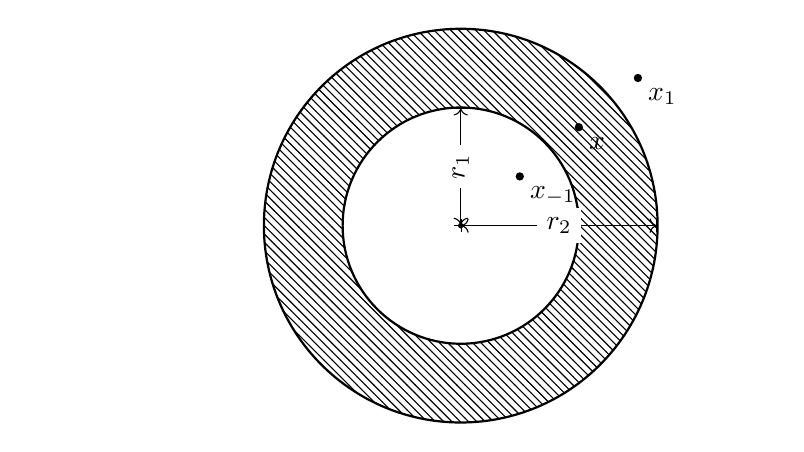
\begin{tikzpicture}[scale=.5]% scale set to 0.5 for explanation %%%

\scope
\clip (-11,-5) rectangle (8,5)
      (0,0) circle (3);
\draw[pattern=north west lines,draw=none] (0,0) circle (5);
\endscope

\fill[thick]  (0,0) circle (2pt);
\fill[thick]  (3,2.5) circle (3pt) node [black,below right] {$x$};
\fill[thick]  (4.5,3.75) circle (3pt) node [black,below right] {$x_1$};
\fill[thick]  (1.5,1.25) circle (3pt) node [black,below right] {$x_{-1}$};
\draw[thick] (0,0) circle (5cm);

\draw[thick] (0,0) circle (3cm);


\draw[|<->|]
            (0,0) -- (5,0) node [midway, fill=white]              {$r_2$};
\draw[|<->|, rotate around with nodes={90:(0,0)}]
            (0,0) -- (3,0) node [midway, fill=white, rotate with] {$r_1$};
\end{tikzpicture}
\end{center}
Let the radius of the inner circle $r_1$ and outer circle $r_2$, and $\Omega=\{x\in \rr^n | r_1<\abs{x}<r_2\}$. We can find points dual to $x$ with respect to inner and outer circle recursively. I'll label dual point inside the inner circle $-$ and outside the outer circle $+$, i.e. $x_1=\frac{r_2^2 x}{\abs{x}^2}$ and $x_{-1}=\frac{r_1^2 x}{\abs{x}^2}$. Recursively, $x_2=\frac{r_2^2 x_1}{\abs{x_1}^2}=\frac{r_2^2}{r_1^2}x$ which is dual point to $x_{-1}$ with respect to outer sphere, and $x_{-2}=\frac{r_1^2 x_{-1}}{\abs{x_{-1}}^2}=\frac{r_1^2}{r_2^2}x$. Then we can easily see that
\begin{equation*}
x_i=
\begin{cases}
\left(\frac{r_2}{r_1}\right)^{i}x & i\equiv 0\Mod{2} \\
\left(\frac{r_2}{r_1}\right)^{(i-1)}r_2^2\frac{x}{\abs{x}^2} & i\equiv 1\Mod{2}\text{ and }i>0 \\
\left(\frac{r_2}{r_1}\right)^{(i+1)}r_1^2\frac{x}{\abs{x}^2} & i\equiv 1\Mod{2}\text{ and }i<0
\end{cases}
\end{equation*}
As $i\rightarrow \infty$, $x_i\rightarrow \infty$ and $i\rightarrow -\infty$, $x_i\rightarrow 0$.

Let's construct Green's function. Let's begin with $G_1(x,y)$:
\begin{equation*}
G_1(x,y)=\Phi(y-x)-\Phi(\frac{\abs{x_0}}{r_2}(y-x_1)).
\end{equation*}
Since $\left(\frac{\abs{x_0}}{r_2}\right)^2\abs{y-x_1}^2=\frac{\abs{x}}{r_2^2}\left(r_2^2-2r_2^2 y\cdot \frac{x}{\abs{x}^2}+r_2^4\frac{1}{\abs{x}^2}\right)=\abs{y-x}^2$, $G_1(x,y)(y)=0$ at $\partial B_{r_2}(x)$.($\Phi$ depends on absolute value of $\abs{y-x}$.)

However, $G_1(x,y)$ is not constant on $\partial B_{r_1}(x)$. To adjust it, we take dual point to $x_0$ and $x_1$ with respect to inner sphere. Set $G_2(x,y)$:
\begin{equation*}
\begin{split}
G_2(x,y)&=\Phi(\frac{\abs{x_0}}{r_1}(y-x_{-1}))-\Phi(\frac{\abs{x_1}}{r_1}\frac{\abs{x_0}}{r_2}(y-x_{-2}))\\
&=\Phi(\frac{\abs{x_0}}{r_1}(y-x_{-1}))-\Phi(\frac{r_2}{r_1}(y-x_{-2}))
\end{split}
\end{equation*}
Then, $\abs{\frac{\abs{x_0}}{r_1}(y-x_{-1})}^2=\abs{y-x}^2$ and
\begin{equation*}
\begin{split}
\frac{\abs{x_1}}{r_1}\frac{\abs{x_0}}{r_2}(y-x_{-2})&=\left(\frac{r_2}{r_1}\right)^2\left(r_1^2-2\left(\frac{r_2}{r_1}\right)^{-2}y\cdot x+\left(\frac{r_2}{r_1}\right)^{-4}\abs{x}^2\right)\\
&=r_2^2-2y\cdot x+\left(\frac{r_2}{r_1}\right)^{-2}\abs{x}^2\\
&=\frac{\abs{x}^2}{r_2^2}\left(r_1^2-2y\cdot r_2^2 \frac{x}{\abs{x}^2}+r_2^4\frac{1}{\abs{x}^2}\right)\\
&=\frac{\abs{x_0}^2}{r_2^2}\abs{y-x_1}^2
\end{split}
\end{equation*}
on $\partial B_{r_1}(x)$. Hence $G_1-G_2=0$ on $\partial B_{r_1}(x)$, but not $0$ on $\partial B_{r_2}(x)$. We can infinitely add $G_i$'s to compensate nonzero term on each sphere. Then, the result will be
\begin{equation*}\label{Eq:7-2}
\begin{split}
G=\sum\limits_{i=1}^\infty (-1)^{i+1} G_i&=\Phi(y-x)+\sum\limits_{i=1}^\infty\left(\Phi(\gamma^i (y-x_{-2i}))+\Phi(\gamma^{-i}(y-x_{2i}))\right) \\
&-\sum\limits_{i=0}^\infty \left(\Phi(\gamma^{-i} \frac{\abs{x}}{r_2}(y-x_{1+2i}))+\Phi(\gamma^i \frac{\abs{x}}{r_1}(y-x_{-1-2i}))\right)
\end{split}
\end{equation*}
where $\gamma\equiv \frac{r_2}{r_1}$. (The final result will be proven later using induction.)

The corrector function is
\begin{equation*}
\phi^x(y)=\sum\limits_{i=1}^\infty\left(\Phi(\gamma^i (y-x_{-2i}))+\Phi(\gamma^{-i}(y-x_{2i}))\right) -\sum\limits_{i=0}^\infty \left(\Phi(\gamma^{-i} \frac{\abs{x}}{r_2}(y-x_{1+2i}))+\Phi(\gamma^{i} \frac{\abs{x}}{r_1}(y-x_{-1-2i}))\right).
\end{equation*}

we need to verify that this corrector function satisfies
\begin{equation*}
\begin{cases}
\Laplace \phi^x=0 & \text{in }\Omega \\
\phi^x=\Phi(y-x) & \text{on }\partial \Omega.
\end{cases}
\end{equation*}

This series for corrector function is convergent since
\begin{equation*}\label{Eq:7-1}
\begin{cases}
\Phi(\gamma^i(y-x_{-2i}))=C(n)\frac{1}{\gamma^i\abs{y-\gamma^{-2i}x}}\leq C(n)\frac{1}{\gamma^i (r_1/2)} & \text{for sufficiently large } i \\
\Phi(\gamma^{-i}(y-x_{2i}))=C(n)\frac{1}{\gamma^{-i}\abs{y-\gamma^{2i}x}}\leq C(n)\frac{2\gamma^i}{\gamma^{2i}\abs{x}} & \text{for sufficiently large } i \\
\Phi(\gamma^{-i}(y-x_{1+2i}))=C(n)\frac{1}{\gamma^{-i}\abs{y-\gamma^{2i}r_2^2 x/\abs{x}^2}}\leq C(n)\frac{2}{\gamma^i r_2^2 x/\abs{x}^2} & \text{for sufficiently large } i \\
\Phi(\gamma^i(y-x_{-2i-1}))=C(n)\frac{1}{\gamma^i\abs{y-\gamma^{-2i}r_1^2 x/\abs{x}^2}}\leq C(n)\frac{1}{\gamma^i (r_1/2)} & \text{for sufficiently large } i. \\
\end{cases}
\end{equation*}
Also, this series is uniformly convergent on $\overline{\Omega}$ and the derivative (w.r.t $y$) is also uniformly convergent; therefore, $\left(\phi^x\right)'(y)$ can be written as infinite sum, and this fact verifies $\phi^x(y)$ is harmonic on $\Omega$.

Considering the construction of the green function and \eqref{Eq:7-1}, $\phi^x(y)$ should be $\Phi(y-x)$ on $\partial \Omega$ since we consistently set the Green's function $0$ on $\partial B_{r_1}(x)$ or $\partial B_{r_2}(x)$, and the added term on another side is converging to $0$, implying the $\phi^x(y)=\Phi(x-y)$ on $\partial B_{r_1}(x)$ and $\partial B_{r_2}(x)$. Therefore, \eqref{Eq:7-2} is the desired Green's function for the the annular region bounded by two concentric spheres in $\rr^n$ for $n \geq 3$.

Now, I'll prove the remained part.
\begin{proposition}
The Green's function for this problem is written as above.
\end{proposition}
\begin{proof}
Let's use induction on $G_i$. I'll show that
\begin{equation*}
G_i=
\begin{cases}
\Phi\left(\gamma^{(-i+1)/2}(y-x_{i-1})\right)-\Phi\left(\gamma^{(-i+1)/2}\frac{|x|}{r_2}(y-x_i)\right) & \text{i is odd} \\
\Phi\left(\gamma^{i/2-1}\frac{\abs{x}}{r_1}(y-x_{-i+1})\right)-\Phi\left(\gamma^{i/2}(y-x_{-i})\right) & \text{i is even}
\end{cases}
\end{equation*}
For $i=0,1$, it is explicitly shown, so let the equation is true for $i\leq k$. If $k$ is odd, then we need to set the Green's function $0$ at $\partial B_{r_1}(x)$. Since
\begin{equation*}
\begin{split}
\abs{\gamma^{(k+1)/2-1}\frac{\abs{x}}{r_1}(y-x_{-k})}^2&=\gamma^{k-1}(\abs{x}^2-2\gamma^{-k+1} y\cdot x+\gamma^{-k+1}r_1^2) \\
&=\gamma^{-k+1}(\gamma^{k-1}x-y)^2 \\
&=\gamma^{-k+1}(x_{k-1}-y)^2
\end{split}
\end{equation*}
and
\begin{equation*}
\begin{split}
\abs{\gamma^{(k+1)/2}(y-x_{-k-1})}^2&=\gamma^{k+1}(r_1^2-2\gamma^{-k-1}y\cdot x + \gamma^{-2k-2}\abs{x}^2) \\
&=\gamma^{-k+1}\frac{\abs{x}^2}{r_2^2}\left(\gamma^{2k+2}\frac{r_1^4}{\abs{x}^2}-\gamma^{k+1}\frac{r_1^2}{\abs{x}^2}y\cdot x+r_1^2\right)\\
&=\gamma^{-k+1}\frac{\abs{x}^2}{r_2^2}(x_k-y)^2,
\end{split}
\end{equation*}
$G_{k+1}=\Phi\left(\gamma^{(k+1)/2-1}\frac{\abs{x}}{r_1}(y-x_{-k})\right)-\Phi\left(\gamma^{(k+1)/2}(y-x_{-k-1})\right)$ for $k$ is odd. By the same way, let $k$ is even, then the Green's function should be $0$ at $\partial B_{r_2}(x)$. Since
\begin{equation*}
\begin{split}
\abs{\gamma^{-k/2}\frac{\abs{x}}{r_2}(y-x_{k+1})}^2&=\gamma^{k}(\abs{x}^2-2\gamma^{-k} y\cdot x+r_2^2) \\
&=\gamma^{k}(\gamma^{-k}x-y)^2 \\
&=\gamma^{k}(x_{-k}-y)^2
\end{split}
\end{equation*}
and
\begin{equation*}
\begin{split}
\abs{\gamma^{-k/2}(y-x_{k})}^2&=\gamma^{-k}(r_2^2-2\gamma^{k}y\cdot x + \gamma^{2k}\abs{x}^2) \\
&=\gamma^{k-2}\frac{\abs{x}^2}{r_1^2}\left(\gamma^{-2k}\frac{r_2^4}{\abs{x}^2}-\gamma^{-k}\frac{r_2^2}{\abs{x}^2}y\cdot x+r_2^2\right)\\
&=\gamma^{k-2}\frac{\abs{x}^2}{r_1^2}(x_{-k+1}-y)^2,
\end{split}
\end{equation*}
$G_k=\Phi\left(\gamma^{(-k+1)/2}(y-x_{k-1})\right)-\Phi\left(\gamma^{(-k+1)/2}\frac{|x|}{r_2}(y-x_k)\right)$ for $k$ is even.

Finally, we need to show that the Green's function is unique. Because $\Phi(y-x)\in C(\partial \Omega)$, there exists at most one solution for correction function, and we just found the solution. Therefore, it is unique.
\end{proof}
\end{document}